% make4ht -ue mybuild.mk4 main_test_file.tex "mathml, mathjax"%

\documentclass[11pt]{article}
\usepackage{amsmath,amssymb,color,float}
\usepackage{stmaryrd}
\usepackage{algorithm}
\usepackage{algpseudocode}
\usepackage{graphicx,psfrag,epsf}
\usepackage[authoryear]{natbib}
\usepackage{fullpage,setspace}
\usepackage{subcaption}
\usepackage{changepage}
\usepackage{listings}
\usepackage{comment}


\newcommand{\rp}{\mathbb{R}^{p_1\times \cdots \times p_M}}
\newcommand{\br}[1]{\llbracket #1 \rrbracket}
\newcommand{\amin}{\operatorname*{argmin}}
\newcommand{\amax}{\operatorname*{argmax}}
\newcommand{\wh}{\widehat}
\newcommand{\wt}{\widetilde} 


\setlength{\oddsidemargin}{.15in} 
\setlength{\textwidth}{6.25in}
\setlength{\topmargin}{-0.25in}
\setlength{\headheight}{-0.15in}
\setlength{\textheight}{8.9in} 

\linespread{1.25}

\title{ST793 Project: A Blogpost on ``Doubly Enhanced EM Algorithm for Model-Based Tensor Clustering" by Mai et al}
\author{Ayumi Mutoh, Jisu Oh, Shih-Ni Prim}

\begin{document}

\maketitle

\section{Introduction}

In recent decades, while tensor data have gained popularity in modern science, their high-dimensional structures often pose challenges for statistical analysis, specifically in model-based clustering. Model-based clustering is a statistical approach to data clustering, where observed data is considered to have been created from a finite combination of component models, such as the Gaussian mixture model (GMM). Since the formalization of the expected-maximization (EM) algorithm by \cite{dempster1977EM}, the EM algorithm has been widely employed in the majority of model-based clustering applications. While the GMMs can be readily extended to higher-order tensors using the standard EM algorithm, their performance can be further enhanced by integrating the Doubly Enhanced EM algorithm (DEEM), as proposed by \cite{mai2022DEEM}. Mai et al. consider a tensor normal mixture model (TNMM) that incorporates tensor correlation structure and variable selection for clustering and parameter estimation. They developed the DEEM algorithm which enables DEEM to excel in high-dimensional tensor data analysis. Similar to the EM algorithm, DEEM carries out an enhanced E-step and an enhanced M-step. 

In this blogpost, we first introduce the DEEM methods with intermediate
steps for the theoretical explanation. The objective is to break down the steps, making the derivation more accessible for our readers to follow. Subsequently, we will conduct a simulation study to evaluate the performance of DEEM.

 
\section{Theoretical Derivation}
\subsection{EM Algorithm}
Before delving into DEEM, we would like to review the EM algorithm and its functioning in clustering.

The EM algorithm is an iterative approach that cycles between two steps for maximum likelihood estimation in the presence of latent variables. The observed data Y is incomplete and data Z is missing. The first step is to write down the joint likelihood, $L_c(
\theta|Y,Z)$, of the ``complete" data $(Y,Z)$. The ``E" step of the EM algorithm is to compute the conditional expectation of log-likelihood, $\text{log}L_c(
\theta|Y,Z)$, given Y, assuming the true parameter value is $\theta^{(\nu)}$
\[Q(\theta,\theta^{(\nu)},Y)=E_{\theta^{(\nu)}}(\text{log}L_c(
\theta|Y,Z)|Y).\] In the ``M" step, we maximize $Q(\theta,\theta^{(\nu)},Y)$ with respect to $\theta$ with $\theta^{(\nu)}$ fixed. We repeat the E step and M step until convergence.  
\begin{comment}
    \begin{itemize}
    \item \textbf{E-step}: Estimate the missing or latent variables  
    \item \textbf{M-step}: Maximize the parameters of the model 
\end{itemize}
\end{comment}

The EM algorithm is well-known for its use in unsupervised learning problems such as clustering with a mixture model. The process goes as follows:
\begin{enumerate}
    \item Identify the number of clusters. 
    \item Define each cluster by generating a Gaussian model. 
    \item For every observation, calculate the probability that it belongs to each cluster (Ex. observation 12 has 40\% probability of belonging to Cluster A and 60\% probability of belonging to Cluster B.)
    \item Use the above probabilities to recalculate the Gaussian models. 
    \item Repeat until observations ``converge" on their assignments. 
\end{enumerate}

Let's consider a simple example. Suppose we have data $X_i$ as shown in Figure \ref{fig:clustering1}, which comes from two distinct classes. We use this data to build a Gaussian model for each class. Since we don't know which class each observation belongs to, there is no straightforward way to construct two Gaussian models to partition the data. Therefore, we begin with a random guess of our Gaussian model parameters: $\mu_1,\sigma^2_1, \mu_2,\sigma^2_2$. 

We have `missing' data points $X_i$ that we believe belong to either of the two distributions. After initializing two random Gaussian models, we compute the likelihood of each observation, $X_i$, being expressed in both of the Gaussian models. The next is the E-step, where we compute the probability that each $X_i$ can belong to any of two distributions. Now we have each point's probability of belonging to either distribution. 

In the M-step, we update the parameters, $\mu_1,\sigma^2_1, \mu_2,\sigma^2_2$, of the model to their most likely values. For the new $\mu_1$, we take a weighted average of all the points, weighted by the probability that they belong to the first distribution. Denoting $p_i$ is the probability that $X_i$ belongs to the first distribution. 
\[\mu_1=\frac{p_1X_1+p_2X_2+\dots+p_nX_n}{p_1+p_2+\dots+p_n}\]
The new $\sigma^2_1$ can be updated similarly. 
\[\sigma^2_1=\frac{p_1(X_1-\mu_1)^2+p_2(X_2-\mu_1)^2+\dots+p_n(X_n-\mu_1)^2}{p_1+p_2+\dots+p_n}\]
We repeat this process for $\mu_2$ and $\sigma^2_2$ and update our distributions. We iterate through the E-step and M-step until convergence, obtaining two clusters as shown in Figure \ref{fig:clustering2}. 




\begin{figure}[H]
    \centering
    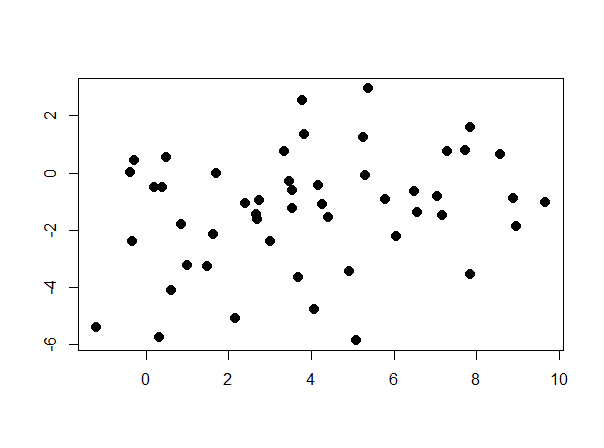
\includegraphics[width = 10 cm]{nocolor.png}
    \caption{Mixture of two Gaussian Distributions}
    \label{fig:clustering1}
\end{figure}


\begin{figure}[H]
    \centering
    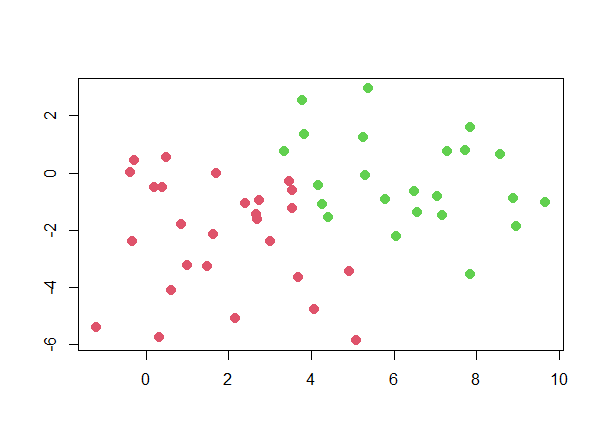
\includegraphics[width = 10 cm]{clustering.png}
    \caption{Clusters Found by EM algorithm}
    \label{fig:clustering2}
\end{figure}


\subsection{Tensor}

While the term ``tensor" might sound unfamiliar to some, tensors are simply multi-way arrays. Data is often structured as matrices, and they are in fact second-order tensors. When we use the term ``tensor," we usually mean tensors of third- and higher-order. The ``order" means the dimension of a tensor, and it is sometimes called the ``mode." You can think of a third-order tensor as a cube. As shown in Figure \ref{fig:tensor}, a tensor can be manipulated similarly as a matrix. In a matrix, we can talk about rows and columns. In a third-order tensor, we can talk about \textbf{fibers} when you fix two modes and keep all values of one mode. The index is then the mode that has all the values. \textbf{Slices} are when you fix one mode and keep all values for the rest of the modes. The index is then the mode that is fixed.

\begin{figure}[H]
    \centering
    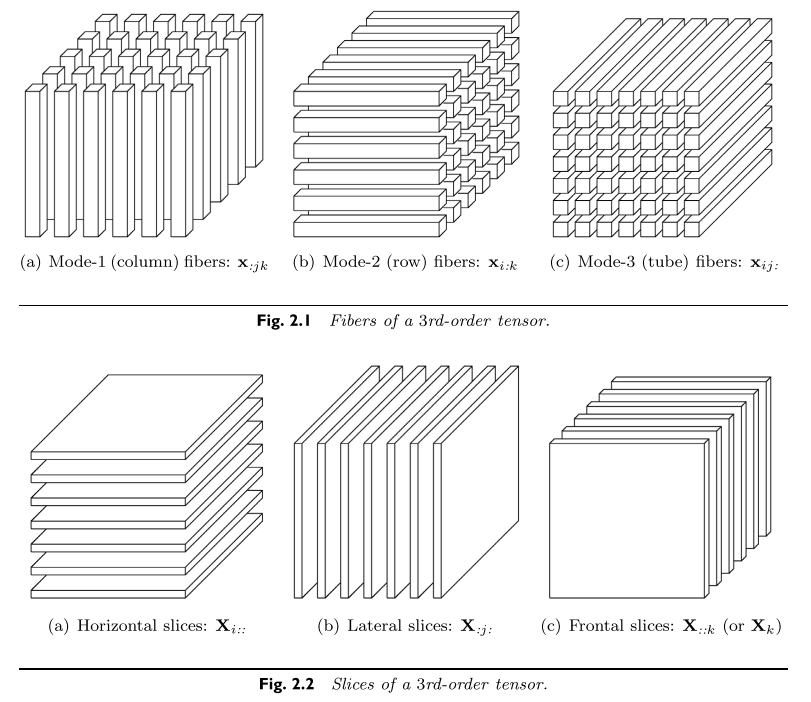
\includegraphics[width = 10 cm]{tensor.png}
    \caption{Dimensions and Terminology of a Tensor, taken from \cite{kolda2009review}}
    \label{fig:tensor}
\end{figure}

Before we continue onto the DEEM algorithm, some concepts and notations are necessary to understand derivations in the following section. Note that the following notations are taken from \cite{kolda2009review}. First of all, we should go over the concept of matricization. If we want to matricize a third-order tensor, we can think of cutting a cube into slices and put the slices side-by-side to make them into a matrix. We now borrow an example (Example 2.1) given in \cite{kolda2009review} to demonstrate how to matricize a third-order tensor $X \in \mathbb{R}^{3\times 4 \times 2}$: 
\begin{equation*}
    X_1 = \begin{bmatrix}
        1 & 4 & 7 & 10 \\ 2 & 5 & 8 & 11 \\ 3 & 6 & 9 & 12 
    \end{bmatrix}, 
    X_2 = \begin{bmatrix} 13 & 16 & 19 & 22 \\ 14 & 17 & 20 & 23 \\ 15 & 18 & 21 & 24  \end{bmatrix}.    
\end{equation*}
The three mode-$n$ unfoldings/matricizations are then
\begin{equation*}
    X_1 = \begin{bmatrix}
        1 & 4 & 7 & 10 & 13 & 16 & 19 & 22 \\ 2 & 5 & 8 & 11 & 14 & 17 & 20 & 23 \\ 3 & 6 & 9 & 12 & 15 & 18 & 21 & 24
    \end{bmatrix},
\end{equation*}
\begin{equation*}
    X_2 = \begin{bmatrix}
        1 & 2 & 3 & 13 & 14 & 15 \\ 4 & 5 & 6 & 16 & 17 & 18 \\ 7 & 8 & 9 & 19 & 20 & 21 \\ 10 & 11 & 12 & 22 & 23  & 24
    \end{bmatrix},
\end{equation*}
\begin{equation*}
    X_3 = \begin{bmatrix}
        1 & 2 & 3 & 4 & 5 & \cdots & 9 & 10 & 11 & 12 \\ 13 & 14 & 15 & 16 & 17 & \cdots & 21 & 22 & 23 & 24 
    \end{bmatrix}.
\end{equation*}
The example above shows that mode-$1$ unfolding is to put $X_1$ and $X_2$ side-by-side and mode-$2$ unfolding is to stack on top of each other. 

This concept is intuitive but much more awkward when we want to define it formally. In \cite{kolda2009review}, the mode-$n$ matricization of a tensor $X \in \mathbb{R}^{I_1 \times I_2 \times \cdots \times I_M}$ is denoted by $X_{(n)}$, which is a matrix of the dimension $(I_n, \prod_{p \ne I_n} I_p)$. (The first dimension comes from the dimension of mode $n$, and the second dimension comes from the product of all the other dimensions.) The tensor element $(i_1, \cdots, i_M)$ is mapped to the matrix element $(i_n, j)$ in the following manner: 
\begin{equation*}
    j = 1 + \sum_{k=1,k\ne n}^M (i_k - 1) J_k \quad \text{with} \quad J_k = \prod_{m=1,m \ne n}^{k-1} I_m.
\end{equation*}
Next, the notation $\llbracket \cdot \rrbracket$ is defined as: 
\begin{equation*}
    \llbracket G; A^{(1)}, A^{(2)}, \cdots, A^{(M)} \rrbracket := G \times_1 A^{(1)} \times_2 A^{(2)} 
    \cdots 
    \times_M A^{(M)},
\end{equation*}
where $A$ are matrices and $X$ and $G$ are tensors. The symbol $\times_n$ means $n$-mode (matrix) product of a tensor $G \in \mathbb{R}^{I_1 \times I_2 \times \cdots \times I_M}$ and the matrices $A^{(n)} \in \mathbb{R}^{J \times I_n}$. $G \times_n A^{(n)}$ is then a tensor of the dimension $I_1 \times \cdots \times I_{n-1} \times J \times I_{n+1} \times \cdots \times I_M$. We can write the elements of $G \times_n A^{(n)}$ as:
\begin{equation*}
    (G \times_n A^{(n)})_{i_1 \, \cdots \, i_{n-1} \, j  \, i_{n+1} \, \cdots \, i_N} = \sum_{i_n = 1}^{I_n} g_{i_1 \, i_2 \, \cdots \, i_N} \cdot a^{(n)}_{j\, i_n}.  
\end{equation*}
Also, for any two tensors $A$ and $B$ in $\mathbb{R}^{I_1 \times I_2 \times \cdots \times I_M}$, we define their inner product by
\begin{equation*}
    \langle A , B \rangle = \sum_{J\in I_1\times I_2 \times \cdots \times I_N} a_J b_J.
\end{equation*}
With that, we are ready to learn about the DEEM algorithm. If you are interested in knowing more about tensors, \cite{kolda2009review} has lots of great details. So be sure to check it out! 

\subsection{Doubly Enhanced EM Algorithm}
In this subsection, we introduce the doubly enhanced EM (DEEM) algorithm and discuss its theoretical properties. Algorithm 1 from \cite{mai2022DEEM} is provided in Appendix as our Figure \ref{fig:deem}.

Let $Z$ denote the random tensor in $\rp$ such that every element in $Z$ is distributed as iid $N(0,1)$.
Then we say that a random tensor $X$ has a tensor normal distribution, denoted by $X\sim \textup{TN}(\mu; \Sigma_1 , \dots, \Sigma_M)$, if $X= \mu+ \br{Z;\Sigma_1^{1/2},\dots, \Sigma_M^{1/2}}$, where $\mu\in \rp$ is the total mean and each $\Sigma_i \in \mathbb{R}^{p_i\times p_i}$ means the covariance matrix within $i$th class. In other words, a tensor normal regression is multivariate normal distribution generalized to a high dimension. An $M^{th}$ order random tensor $X$ has a total of $\sum_{i=1}^M p_i$ means and $M$ covariate matrices each of the dimension $p_i \times p_i$ for $i = 1, \cdots, M$. We can find that the density of $X$ has the form
\begin{equation}\label{density}
  p(X|\mu; \Sigma_1 , \dots, \Sigma_M) = \frac{1}{(2\pi)^{p/2} |\Sigma_1|^{q_i/2}\cdots |\Sigma_M|^{q_M/2}} \exp\left( -\frac{1}{2} \left\langle \br{X-\mu; \Sigma_1^{-1}, \dots, \Sigma_M^{-1}}, X-\mu \right\rangle  \right),
\end{equation}
where $p=p_1p_2 \cdots p_M$ and $q_i=p/p_i$. 

We will consider independent tensor-variate observations in $\mathbb{R}^{p_1,\times \cdots \times p_M}$ drawn from $K$ clusters with the same within-class covariance matrices; suppose that $\mu_i$'s are the mean tensor of the $k$th cluster. Let $\pi_k$ be the probability of an observation to be taken from the $k$th cluster. 

Then  the sample $\{X_i\}_{i=1}^n$ from a mixture of the tensor normal distributions can be written as the following:
\begin{equation*}
  X_i \sim \sum_{k=1}^K \pi_k\textup{TN}(\mu_k ; \Sigma_1 ,\dots, \Sigma_M), \quad i=1,2,\dots, n,
\end{equation*}
or equivalently,
\begin{equation}\label{model}
  P(Y_i=k)=\pi_k \and X_i|Y_i=k \sim \textup{TN}(\mu_k; \Sigma_1, \dots, \Sigma_M), \quad i=1,2,\dots, n.
\end{equation}
Hence, $Y_i$ indicates the number of the cluster from which $X_i$ was taken, and if $Y_i=k$ is given, $X_i$ has the tensor normal distribution with the mean $\mu_k$ of the cluster $k$ and the within-class covariance matrices $\Sigma_1,\dots, \Sigma_M$. (Recall we assume that the clusters have the same within-class matrices.) 




Suppose that $\{X_i\}_{i=1}^n$ is a sample from the model \eqref{model}. Let $\theta=\{\pi_i, \mu_i, \Sigma_j: 1\le i \le K, 1\le j \le M\}$ denote the set of all parameters in the model.
If we can observe $Y_i$, then the complete log-likelihood can be obtained as follows:
\begin{align*}
  \ell_c (\theta;X,Y) = \log \prod_{i=1}^n \pi_{Y_i} p(X_i|\mu_{Y_i};\Sigma_1,\dots \Sigma_M)=  \sum_{i=1}^n [\log\pi_{Y_i}+ \log p(X_i| \mu_{Y_i}, \Sigma_1,\dots , \Sigma_M)].
\end{align*}
But, in general, we cannot observe $Y_i$; hence, from an initial value $\wt\theta^{(0)}$, we create a sequence $\wt\theta^{(t)}$ through the E-step to obtain the $Q$ function
\begin{equation*}
 Q(\theta; \wt\theta^{(t)}) = E_{Y|X,\wt\theta^{(t)}}[\ell_c(\theta;X,Y)] = \sum_{i=1}^n \sum_{k=1}^K \wt \xi_{ik}^{(t)} [ \log \pi_k + \log p(X_i | \mu_k , \Sigma_1,\dots \Sigma_M)]
\end{equation*}
where
\begin{equation}\label{Estep}
  \wt\xi _{ik}^{(t)} = P(Y_i=k| X,\wt\theta^{(t)}) = \frac{\wt\pi_k^{(t)} p(X_i|\wt \mu_k^{(t)}, \wt\Sigma_1^{(t)},  \dots, \wt \Sigma_M^{(t)})}{\sum_{j=1}^K \wt\pi_j^{(t)} p(X_i | \wt\mu_j^{(t)}, \wt\Sigma_1^{(t)}, \dots, \wt\Sigma_M^{(t)})}
\end{equation}
and the M-step to update the parameter
\begin{equation*}
	\wt\theta^{(t+1)} = \amax_\theta Q(\theta; \wt\theta^{(t)}).
\end{equation*}
Then the EM sequence $\wt\theta^{(t)}$ converges to the MLE, but there are some issues in our situation:
Getting the updates for $\pi_k$ and $\mu_k$ is quite easy and straightforward, but it is challenging to obtain the updates for the covariance matrices $\Sigma_i$.
When we compute $\wh\xi^{(t)}_{ik}$ in \eqref{Estep}, all the elements in $X_i$ are used, and the standard EM algorithm does not involve a process for variable selection.
Thus, due to an excessive number of parameters in the model, it may lead to the accumulation of errors, which potentially resulting in inaccurate estimates.




To overcome these problems, we introduce the enhanced E-step, where we replace $\wt\xi^{(t)}_{ik}$ with an estimator $\wh\xi^{(t)}$ that can be calculated relatively faster under the sparsity assumption. 
We want to find the objective function $Q^{\textup{DEEM}}$ that has a better property than the standard $Q$ function above. First, it can be seen that
\begin{equation}\label{xi1}
  \xi_{i1}=P(Y_i=1|X_i, \theta) = \frac{\pi_1}{\pi_1 + \sum_{k=2}^K \pi_k \exp\left[ \langle X_i - (\mu_k+\mu_1)/2 , B_k \rangle \right]}
\end{equation}
and
\begin{equation}\label{xi2}
  \xi_{ik}=P(Y_i=k|X_i, \theta) = \frac{\pi_k \exp \left[ \langle X_i - (\mu_k+\mu_1)/2 , B_k \rangle \right]}{\pi_1 + \sum_{j=2}^K \pi_j \exp\left[ \langle X_i - (\mu_j+\mu_1)/2 , B_j \rangle \right]}
\end{equation}
for $k\ge2$, where
\begin{equation*}
  B_k = \br{\mu_k - \mu_1 ; \Sigma_1^{-1} , \dots , \Sigma_M^{-1}}\in  \rp.
\end{equation*}
Note that we are considering the clustering problem, that is, we are interested in recovering $Y_i$'s and finding a method that minimizes the clustering error.
It can be shown that the covariance matrices $\Sigma_i$ are nuisance parameters in the optimal clustering rule, i.e., 
the values of $\Sigma_i$ are not used in the optimal clustering rule if we already know $B_k$'s.
To cover more general cases, we do not impose conditions on $\Sigma_i$.
Instead, we assume the sparsity condition on $B$; for $B_k=[b^J_k]_{J}$, where $J=(j_1,\dots, j_M)$ denotes an index of the tensor, we impose the condition $b_2^J=\cdots = b_K^J=0 $ for almost every $J$. In other words, if 
$D= \{J : b_k^J \neq 0 \text{ for some $k=2,\dots, K$} \}$, then we assume that the number of elements in $D$ is significantly smaller than $p=p_1p_2 \cdots p_M$. This assumption comes from the belief that, in the high-dimensional setting, most of variables are not significant in estimation.
The above expressions for $\xi_{ik}$ show that this assumption reduces the computational cost and improves the  estimation efficiency.





If we accept the fact that $(B_2,\dots, B_K)$ minimizes the quantity
\begin{equation*}
  \sum_{k=2}^K  \left( \langle B_k , \br{B_k, \Sigma_1 , \dots , \Sigma_M} \rangle - 2 \langle B_k , \mu_k - \mu_1 \rangle \right),
\end{equation*}
then it is reasonable to obtain the sequence of estimates $\wh B_k^{(t+1)}$ by solving the optimization problem
\begin{equation*}
  \amin_{B_2,\dots, B_K}\sum_{k=2}^K  \left( \langle B_k , \br{B_k, \wh\Sigma_1^{(t)} , \dots , \wh \Sigma_M^{(t)}} \rangle - 2 \langle B_k , \wh \mu_k ^{(t)}- \wh \mu_1^{(t)} \rangle \right) + \lambda^{(t+1)}\sum_J \left( \sum_{k=2}^K (b_k^J)^2 \right),
\end{equation*}
where we added the lasso penalty term to satisfy the sparsity assumption to some extent.
Using these $\wh B_k^{(t+1)}$, we can obtain the sequence $\wh\xi^{(t+1)}_{ik}$ by replacing the parameters in \eqref{xi1} and \eqref{xi2} with their estimates.
Then, the objective $Q^{\textup{DEEM}}$ is defined using $\wh\xi^{(t)}$ as follows:
\begin{equation*}
  Q^{\textup{DEEM}}(\theta; \wh\theta^{(t)}) = \sum_{i=1}^n \sum_{k=1}^K \wh \xi^{(t)}_{ik}[\log \pi_k +\log p(X_i| \mu_k , \Sigma_1, \dots , \Sigma_M)].
  \end{equation*}

In light of the sparsity assumption, $\wh\xi^{(t)}_{ik}$ can be computed based on the values of relatively smaller variables.


In M-step, the parameters can be updated inductively from the proposed $Q^{\textup{DEEM}}$ function:
The estimates for $\pi_k$ and $\mu_k$ can be obtained by the formula
\begin{equation*}
  \wh\pi_k^{(t+1)} = \frac{1}{n}\sum_{i=1}^n \wh\xi_{ik}^{(t+1)} \quad\text{and}\quad \wh\mu_k^{(t+1)} = \frac{\sum_{i=1}^n \wh\xi_{ik}^{(t+1)}X_i}{\sum_{i=1}^n \wh\xi_{ik}^{(t+1)}} ,\quad k=1,2,\dots, K.
\end{equation*}
Then given $\xi_{ik}^{(t+1)}$, we calculate the intermediate covariance matrices
\begin{equation*}
  \overset  \smile \Sigma^{(t+1)}_j = \frac{1}{nq_j} \sum_{i=1}^n \sum_{k=1}^K \wh\xi^{(t+1)}_{ik} (X_i - \wh\mu_k^T{(t+1)})_{(j)} (X_i - \wh\mu_k^T{(t+1)})_{(j)} ^T,
\end{equation*}
and the conditional variance of $X_i^{1\dots1}$
\begin{equation*}
  (\wh\sigma_{1}^{11})^{(t+1)} = \frac{1}{n}\sum_{i=1}^n \sum_{k=1}^K \wh\xi_{ik}^{(t+1)} (X_i^{1\dots1}-(\wh \mu_{k}^{1\dots1})^{(t+1)})^2.
\end{equation*}
The target covariance estimator is given by scaling the intermediate covariances with $(\wh\sigma_{1}^{11})^{(t+1)}$ and $(\overset \smile \sigma_1^{11})^{(t+1)}$:
\begin{equation*}
  \wh \Sigma_j^{(t+1)} =
  \left\{
  \begin{aligned}
  	&\frac{1}{(\overset \smile \sigma_j^{11})^{(t+1)}}\overset \smile \Sigma_j^{(t+1)} \quad \text{if $j\ge 2$}, \\
  	&\frac{(\wh \sigma_1^{11})^{(t+1)}}{(\overset \smile \sigma_1^{11})^{(t+1)}}\overset \smile \Sigma_1^{(t+1)} \quad \text{if $j= 1$}.
  \end{aligned}
  \right.
\end{equation*}
The general process is summarized in Algorithm 1 in Appendix as our Figure \ref{fig:deem}.

Now we are interested in how this sequence of parameters $\wh\theta^{(t)}$ behave.
In fact, under some initialization condition, it can be seen that there are some constant $C$ and $0<\kappa<1/2$ such that for large $t$, with a probability $\ge 1- O(\prod_{i=1}^M p_i^{-1})$,
$$
\|\wh B^{(t)} - B\| \le C\sqrt{\frac{s \Sigma_{i=1}^M \log p_i}{n}},
$$
where $s=o(\sqrt{n/\sum_i \log p_i})$ and $d_0$ is a measure of the difference between the initial value $\wh \theta^{(0)}$ and the true parameter $\theta$.
This result implies that if the number of iterations $t$ is large, the DEEM estimator $\wh B^{(t)}$ converges to the true parameter $B$.
Here, the condition $s=o(\sqrt{n/\sum_i \log p_i})$ means the sparsity assumption.

We consider the error rate of DEEM and the optimal clustering rule:
$$
R(DEEM)= \min_{\Pi} P(\Pi(\wh Y_i^{DEEM} \neq Y_i)) \quad\text{and}\quad R(Opt)= P(\wh Y_i^{opt} \neq Y_i),
$$
where $\Pi$ denotes the permutation operator and $\wh Y_i^{DEEM}= \amax_k \wh\xi_{ik}$.
Here, the optimal clustering rule is optimal in the sense that it minimizes the clustering error.
From the result above, we can show that if $t$ is large, then with probability $\ge 1- O(\prod_{i=1}^M p_i^{-1})$
$$
R(DEEM) - R(Opt) \le C \frac{s\sum_{i=1}^M \log p_i}{n}.
$$
Consequently, this result shows that the error rate of DEEM converges to the error rate of the optimal clustering rule if $t$ is large.


\section{Simulation Study}

\subsection{Data Generation}

For our simulation studies, we follow the framework used in \cite{mai2022DEEM}. For each setting, $K$ denotes the number of mixture groups, and noise is generated as a $M^{th}$-order tensor:  
\begin{equation}
    \mathbf{X}_i \sim \sum_{k=1}^K \pi^*_k \mbox{TN} (\boldsymbol{\pi}^*_k; \boldsymbol{\Sigma}^*_1, \cdots, \boldsymbol{\Sigma^*_M}), i = 1, \cdots, n
\end{equation}
For $K-1$ mixture groups, the $\mathbf{X}_i$ is given as a given $\mathbf{B}_k$ plus the noise above. For $1$ mixture group, the values are simply the noise. \citeauthor{mai2022DEEM} designate two types of $\boldsymbol{\Sigma}^*_k$: 
\[  \boldsymbol{\Omega} =   \begin{cases}
     AR(\rho): & \omega_{ij} = \rho^{|i-j|} \\
    CS(\rho): & \omega_{ij} = \rho + (1-\rho) 1(i=j).
\end{cases}\]
The covariance matrices are not sparse if they are set using the two formats above. For each setting, we generate $100$ independent datasets, the same number of replicates as used by the authors, and present the mean error rate and standard deviation. 

\subsection{Settings}

The settings are provided in Table \ref{tab:sim_setting}. Note that, for ${B}^*_{k}$, the indices not included in the subscript is $0$. In other words, ${B}^*_k$ is a sparse tensor. Both the DEEM and EM algorithms require $K$ to be given. $\lambda$ is a tuning parameter for regularization; however, due to the long computation time, we experiment with several different values of $\lambda$ and set it at $0.05$ instead of tuning it for each setting. We encourage the interested readers to try out two functions--\textbf{tune\_K} and \textbf{tune\_lambda}--in the R package \textbf{TensorClustering}. 

We choose four settings from the seven settings, because these settings are increasingly more computationally expensive, and we believe that they demonstrate the advantage of the DEEM algorithm compared to the classical EM algorithm in terms of accuracy, as shown in Table \ref{tab:err}. We also run three extra settings, which we call M8, M9, M10 to avoid confusion with the seven settings in the paper. The results for these extra settings are shown in Tables \ref{tab:err2} and \ref{tab:time2}.

\begin{table}[H]
    \centering
    \begin{tabular}{|c|p{4in}|}
    \hline
      Model & Parameters \\
    \hline
    M1  & $K=2, p = 10\times 10 \times 4, \boldsymbol{\Sigma}^*_1 = CS(0.3), \boldsymbol{\Sigma}^*_2 = AR(0.8), \boldsymbol{\Sigma}^*_3 = CS(0.3), \mathbf{B}^*_{2,[1:6,1,1]} = 0.5$  \\
    \hline
    M3 &  $K=3, p = 10\times 10 \times 4, \boldsymbol{\Sigma}^*_1 = CS(0.3), \boldsymbol{\Sigma}^*_2 = AR(0.8), \boldsymbol{\Sigma}^*_3 = CS(0.5), \mathbf{B}^*_{2,[1:6,1,1]} = 0.5, \mathbf{B}^*_{3,[1:6,1,1]} = -0.5$  \\
    \hline
    M4 &  $K=4, p = 10\times 10 \times 4, \boldsymbol{\Sigma}^*_1 = \mathbf{I}_{10}, \boldsymbol{\Sigma}^*_2 = AR(0.8), \boldsymbol{\Sigma}^*_3 = \mathbf{I}_4, \mathbf{B}^*_{2,[1:6,1,1]} = 0.8, \mathbf{B}^*_{3,[1:6,1,1]} = -0.8$ \\
    \hline
    M5 &  $K=6, p = 10\times 10 \times 4, \boldsymbol{\Sigma}^*_1 = AR(0.9), \boldsymbol{\Sigma}^*_2 = CS(0.6), \boldsymbol{\Sigma}^*_3 = AR(0.9), \mathbf{B}^*_{2,[1:6,1,1]} = 0.6, \mathbf{B}^*_{3,[1:6,1,1]} = 1.2, \mathbf{B}^*_{4,[1:6,1,1]} = 1.8, \mathbf{B}^*_{5,[1:6,1,1]} = 2.4, \mathbf{B}^*_{6,[1:6,1,1]} = 3$ \\
    \hline
    M8 & $K=2, p = 10 \times 10 \times 10, \boldsymbol{\Sigma}^*_1 = AR(0.5), \boldsymbol{\Sigma}^*_2 = CS(0.5), \boldsymbol{\Sigma}^*_3 = AR(0.5), \mathbf{B}^*_{2,[1:3,1,1]} = 5$\\
    \hline
    M9 & $K=2, p = 10 \times 10 \times 10, \boldsymbol{\Sigma}^*_1 = \mathbf{I}_{10}, \boldsymbol{\Sigma}^*_2 = \mathbf{I}_{10}, \boldsymbol{\Sigma}^*_3 = \mathbf{I}_{10}, \mathbf{B}^*_{2,[1:3,1,1]} = 3$ \\ 
    \hline
    M10 & $K=2, p = 10 \times 10 \times 4 \times 4 \times 4, \boldsymbol{\Sigma}^*_1 = AR(0.5), \boldsymbol{\Sigma}^*_2 = CS(0.5), \boldsymbol{\Sigma}^*_3 = AR(0.5), \boldsymbol{\Sigma}^*_4 = \mathbf{I}_4, \boldsymbol{\Sigma}^*_5 = \mathbf{I}_4, \mathbf{B}^*_{2,[1:3,1,1]} = 5$ \\
    \hline
    \end{tabular}
    \caption{Simulation settings}
    \label{tab:sim_setting}
\end{table}

\subsection{Metrics}

Note that it is as straightforward to calculate the mean error rate for a clustering problem than it is for a classification problem. Both methods return labels for the groups; however, the group labels do not matter. For example, if there are five observations and if their true group labels are $(1,1,2,2,2)$ and the methods return $(2,2,1,1,1)$, the error rate should be $0$. In the paper, the authors explain that mean clustering error rate is calculated by: 
\[ \min_\Pi \frac{1}{n} \sum_{i=1}^n 1 (\hat{Y}_i \ne \Pi (Y_i)) \text{ over all possible permutations } \Pi: \{1, \cdots,  \} \mapsto \{1, \cdots, K\} \]
We create a function to permute the true labels, compare the estimated labels and the true labels, and return the lowest error rate. To compare the speed of the two methods, we also record the computation time. Table \ref{tab:time} provides the mean computation time and standard error (in parentheses) for each setting. 

\subsection{External R Packages and Functions}

For the DEEM algorithm, we use the function DEEM; for the standard EM algorithm, we use the function TGMM. Both functions are from the R package TensorClustering. We use the Trnorm function from the R package Tlasso to generate tensor noise with designated covariance matrices. We use the permutations function in the gtools package to permute true labels. In short, be sure to install the three R packages: TensorClustering, Tlasso, and gtools if you would like to reproduce our simulation. 


\subsection{Simulation result}

The error rates and computation time are shown in Tables \ref{tab:err} and \ref{tab:time}. It is clear that DEEM has lower mean error rates in all four settings. The error rates are in general higher than those given in the article, possibly because the hyperparameters are not tuned for each setting in our case.

The computation time tells a different story, however. As seen in Table \ref{tab:time}, DEEM is not always the winner in terms of time. As the setting becomes more complicated and estimating the clusters becomes more challenging, it takes longer for DEEM to converge. For setting M5, it is possible that DEEM reached the maximum iterations for some runs. 

\begin{table}[H]
    \centering
    \begin{tabular}{|c|cc|}
    \hline
       Model  &  DEEM & EM \\
       \hline
         M1 & 0.41 (0.05) & 0.45 (0.03) \\
         M3 &  0.46 (0.09) & 0.56 (0.05) \\
         M4 &  0.35 (0.03) & 0.57 (0.06) \\ 
         M5 &  0.31 (0.11) & 0.43 (0.06) \\
    \hline
    \end{tabular}
    \caption{Error Rates from 100 Replicates}
    \label{tab:err}
\end{table}

\begin{table}[H]
    \centering
    \begin{tabular}{|c|cc|}
    \hline
       Model  &  DEEM & EM \\
       \hline
         M1 & 0.72 (0.45) & 0.93 (0.39) \\
         M3 &  13.95 (7.78) & 7.74 (3.99) \\
         M4 &  15.8 (0.81) & 21.9 (9.68) \\ 
         M5 &  332.96 (124.38) & 14.66 (5.88) \\
    \hline
    \end{tabular}
    \caption{Computation Time (seconds) from 100 Replicates}
    \label{tab:time}
\end{table}

Next we transform the values in the tables into figures. As shown in Figure \ref{fig:err}, DEEM always has lower mean error rates. However, as the model becomes complicated, DEEM's error rates become more varied, even though the mean rate is still lower. In Figure \ref{fig:time}, the story seems more complicated. (Note that we cannot use the same y-axis for all four plots, because the computation time for DEEM for M5 is so long, which would make some of the boxes very small and not informative.) For the two settings M1 and M4, DEEM has lower computation time. For M3, the computation time for DEEM is much more varied, and EM has overall shorter computation time. For M5, DEEM has very long computation time; in fact, the 100 replicates took almost 10 hours. It is unclear if the reduced error rate is worth the computational cost.

\begin{figure}[H]
    \centering
    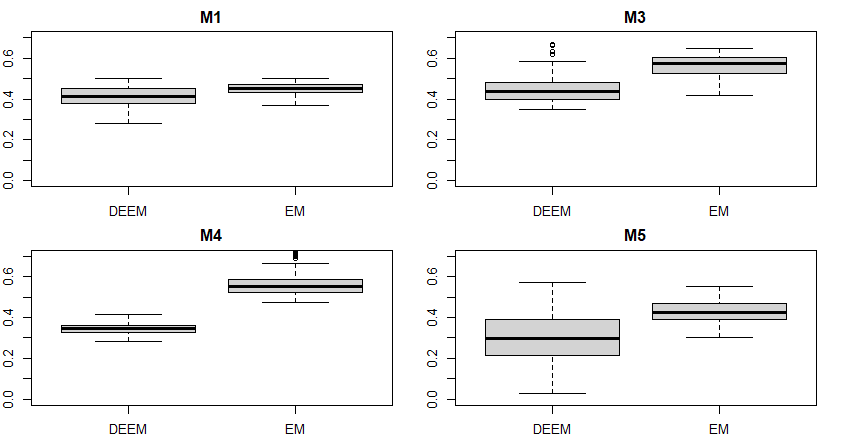
\includegraphics[width = 16 cm]{sim_error.png}
    \caption{Boxplots of Mean Error Rates from 100 Replicates}
    \label{fig:err}
\end{figure}

\begin{figure}[H]
    \centering
    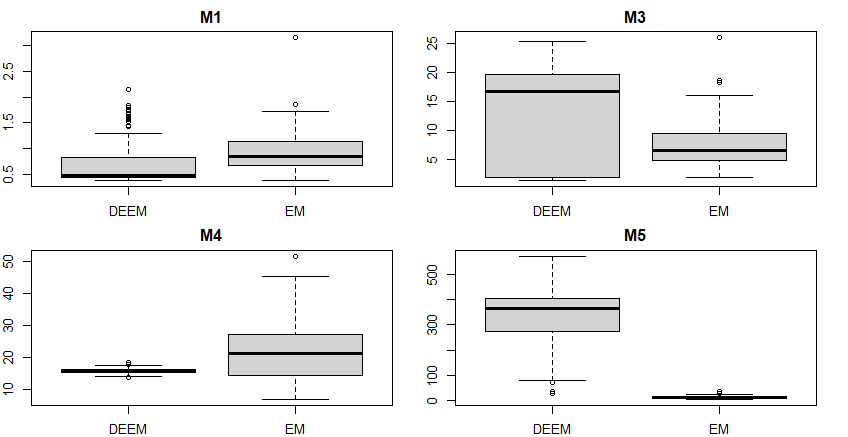
\includegraphics[width = 16 cm]{sim_time.png}
    \caption{Boxplots of Mean Computation Time (in seconds) from 100 Replicates}
    \label{fig:time}
\end{figure}

In terms of the extra settings, we noticed that the error for DEEM is much lower than EM for M8, for which we set $2$ clusters with the covariance matrices to have moderate correlation. This setting allows DEEM to really outperform EM, perhaps because it is just complicated enough to mess up the performance of the EM algorithm. For M9, we let the setting to be an easy case, since the covariance matrices are all identity matrices. As expected, the error rates are quite similar. For M10, we use a fifth-order tensor. [add here]

\begin{table}[H]
    \centering
    \begin{tabular}{|c|cc|}
    \hline
       Model  &  DEEM & EM \\
       \hline
         M8 & 0.02 (0.10) & 0.33 (0.19) \\
         M9 &  0.03 (0.01) & 0.06 (0.03) \\
         M10 &  0.xx (xxx) & 0.xx (xxx) \\ 
    \hline
    \end{tabular}
    \caption{Error Rates from 100 Replicates}
    \label{tab:err2}
\end{table}

\begin{table}[H]
    \centering
    \begin{tabular}{|c|cc|}
    \hline
       Model  &  DEEM & EM \\
       \hline
         M8 & 3.25 (7.62) & 0.44 (0.37) \\
         M9 &  4.41 (0.88) & 0.14 (0.02) \\
         M10 &  xx.xx (xxx) & xx.xx (xxx) \\ 
    \hline
    \end{tabular}
    \caption{Computation Time (seconds) from 100 Replicates}
    \label{tab:time2}
\end{table}

\section{Summary}

In this blogpost, we review a new method proposed by \cite{mai2022DEEM}, which is essentially an upgraded version of the classical EM algorithm. This new method, DEEM, tends to have lower error rates on tensor data. However, despite the paper's claim that the enhanced M step in the DEEM algorithm facilitates fast covariance estimation, we have encountered situations where the running time could be prohibitive. While DEEM proves to be efficient and effective in handling tensor data, there remains potential for further enhancement.


\begin{singlespace}
	\bibliographystyle{rss}
	\bibliography{refs}
\end{singlespace}

\section*{Appendix}
\begin{figure}[H]
    \centering
    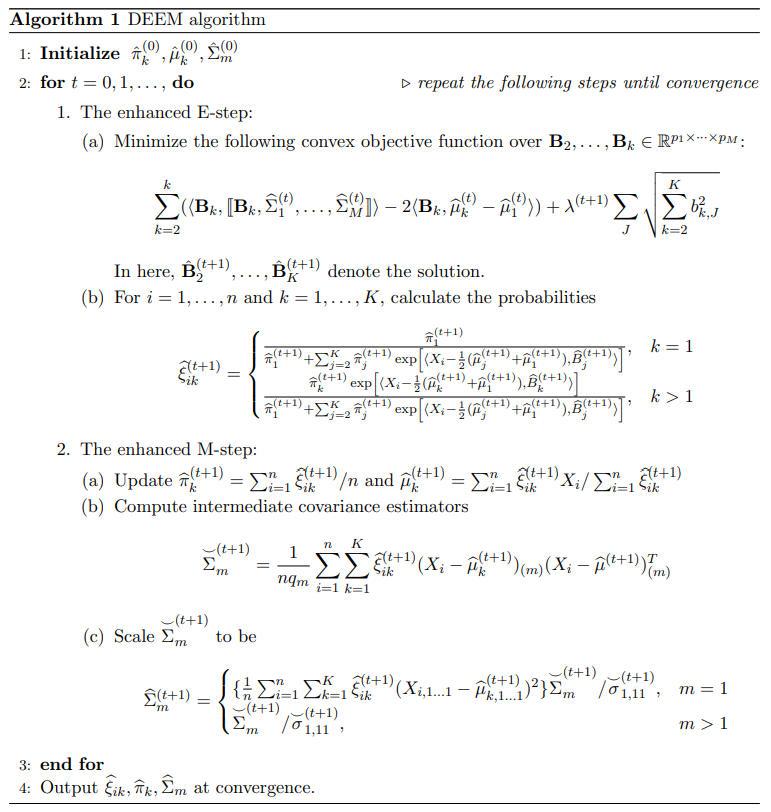
\includegraphics[width = 16 cm]{deem.png}
    \caption{DEEM algorithm}
    \label{fig:deem}
\end{figure}



\begin{comment}
\algblock{Input}{EndInput} %Helper for writing input for algorithm
\algblock{Initialize}{EndInitialize} %Helper for writing initial values for algorithm
\algnotext{EndInput} %Hide the end statement since it's ugly and unnecessary
\algnotext{EndInitialize}


\begin{algorithm}
    \caption{DEEM algorithm}\label{alg:DEEM}
    \begin{algorithmic}[1]
       \Initialize \; \(\hat{\pi}^{(0)}_k, \hat{\mu}^{(0)}_k, \hat{\Sigma}^{(0)}_m\)
       \EndInitialize
       \For {$t=0,1,\dots,$} \Comment{\textit{repeat the following steps until convergence}}
       \begin{enumerate}
           \item The enhanced E-step: 
           \begin{enumerate}
               \item Minimize the following convex objective function over \(\mathbf{B}_{2},\dots,\mathbf{B}_k\in \mathbb{R}^{p_1\times \dots \times p_M}\):
               \[\sum^k_{k=2}(\langle\mathbf{B}_k,\llbracket\mathbf{B}_k,\wh\Sigma^{(t)}_1,\dots,\wh\Sigma^{(t)}_M\rrbracket\rangle-2\langle\mathbf{B}_k,\wh\mu^{(t)}_k-\wh\mu^{(t)}_1\rangle)+\lambda^{(t+1)}\sum_J\sqrt{\sum^K_{k=2}b^2_{k,J}}\]
               In here, \(\hat{\mathbf{B}}^{(t+1)}_2,\dots,\hat{\mathbf{B}}^{(t+1)}_K\) denote the solution. 
               \item For \(i=1,\dots,n\) and \(k=1,\dots,K\), calculate the probabilities 
               \[ \wh\xi_{ik}^{(t+1)}=\begin{cases}
                    \frac{\wh\pi_1^{(t+1)}}{\wh\pi_1^{(t+1)} + \sum_{j=2}^K \wh \pi_j ^{(t+1)}  \exp\left[ \langle X_i - \frac{1}{2}(\wh \mu_j^{(t+1)} +\wh \mu_1^{(t+1)} ) , \wh B_j^{(t+1)}  \rangle \right]}, & k=1\\
                    \frac{\wh\pi_k^{(t+1)}\exp\left[ \langle X_i - \frac{1}{2}(\wh \mu_k^{(t+1)} +\wh \mu_1^{(t+1)} ), \wh B_k^{(t+1)}  \rangle \right]}{\wh\pi_1^{(t+1)} + \sum_{j=2}^K \wh \pi_j ^{(t+1)}  \exp\left[ \langle X_i - \frac{1}{2}(\wh \mu_j^{(t+1)} +\wh \mu_1^{(t+1)} ) , \wh B_j^{(t+1)}  \rangle \right]}, & k>1
               \end{cases}\]
           \end{enumerate}
           \item The enhanced M-step:
               \begin{enumerate}
                   \item Update \(\wh\pi^{(t+1)}_k=\sum^n_{i=1}\wh\xi^{(t+1)}_{ik}/n\) and \(\wh\mu^{(t+1)}_k=\sum^n_{i=1}\wh\xi^{(t+1)}_{ik}X_i/\sum^n_{i=1}\wh\xi^{(t+1)}_{ik}\)
                   \item Compute intermediate covariance estimators 
                   \[\overset\smile\Sigma^{(t+1)}_m=\frac{1}{nq_m}\sum^n_{i=1}\sum^K_{k=1}\wh\xi^{(t+1)}_{ik}(X_i-\wh\mu^{(t+1)}_k)_{(m)}(X_i-\wh\mu^{(t+1)})^T_{(m)}\]
                   \item Scale \(\overset\smile\Sigma^{(t+1)}_m\) to be 
                   \[\wh\Sigma^{(t+1)}_m=\begin{cases}
                       \{\frac{1}{n}\sum^n_{i=1}\sum^K_{k=1}\wh\xi^{(t+1)}_{ik}(X_{i,1\dots1}-\wh\mu^{(t+1)}_{k,1\dots 1})^2\}\overset\smile\Sigma^{(t+1)}_m/\overset\smile\sigma^{(t+1)}_{1,11}, & m=1\\
                       \overset\smile\Sigma^{(t+1)}_m/\overset\smile\sigma^{(t+1)}_{1,11}, & m>1
                   \end{cases}\]
               \end{enumerate}
       \end{enumerate}
        \EndFor
        \State Output \(\wh\xi_{ik}, \wh\pi_k, \wh\Sigma_m\) at convergence.
    \end{algorithmic}
\end{algorithm}
\end{comment}

\end{document}